\subsection{OSI - Network Layer}

	\defn{End-to-End Principle}{is a network design principle whereby application-specific features reside in the end nodes, rather than being distributed across the network}

	\par{The Network layer is responsible for end-to-end delivery of data and is therefore the first end-to-end layer in the OSI. This is important because networks can be of enourmous sizes, and since implementing a function always has a cost, if that function is implemented across the whole of the network that cost quickly multiplies. If instead the system is concerned with achieving reliability of communication above a certain threshold, it is more efficient to implement processes for checking for correctness and completeness at the end hosts rather than at the intermediary nodes, since end-to-end reliability is not perfectly aligned with the reliability of intermediary processes}

	\defn{Internet}{set of interconnect networks}

	\defn{Autonomous System}{a network within a larger network which is administered separately by a single organisation who is responsible for making independent policy and technology choices}

	\par{The basic components of an internet are:}

	\begin{enumerate}
		\item The existence of a common end-to-end protocol, which provides a single seamless service to the transport layer
		\item A set of intermediate gateway devices, i.e routers, which implement the protocol and hide differences in link layer technologies by performing the usual services provide by that layer
	\end{enumerate}

	\subsection{Network Layer - Internet Protocol}

	\par{The IP provides an abstraction layer, including a \ita{simple, best effort, connectionless} packet delivery service. Which means, that it does not guarantee correctness or delivery, but it allows for addressing, routing, fragmentation and reassembly of packets.}
	\par{The IP service model does not require a connection to be setup first, instead it just sends the available packets and anything which cannot be delivered is discarded. This means that it favours simplicity over assurance and correctness, leaving that for the layers above.}

			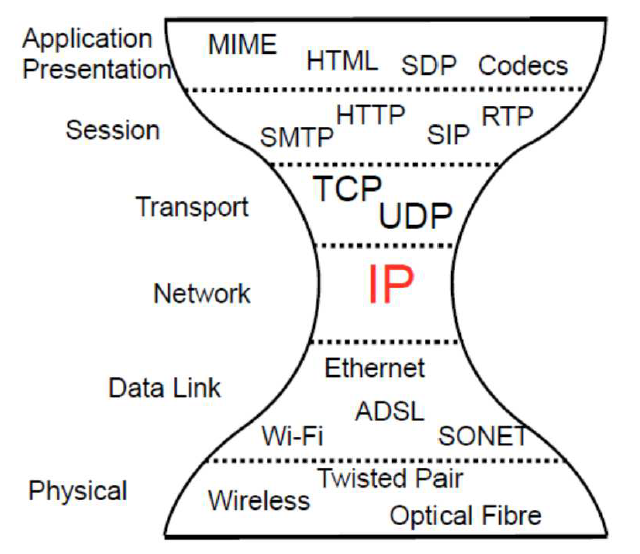
\includegraphics[height=0.3\textheight]{protocols.png}

			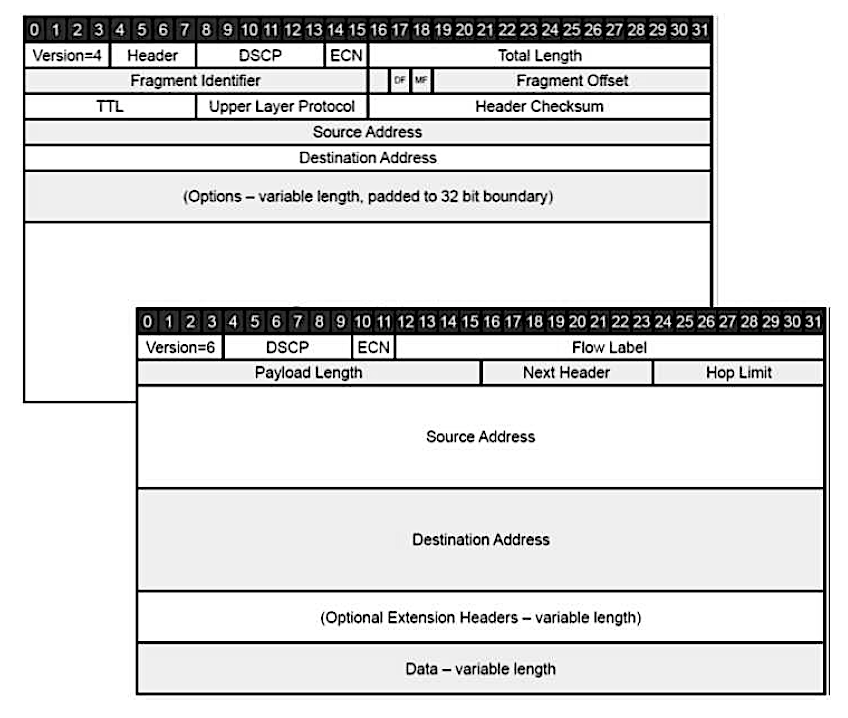
\includegraphics[width=0.7\textwidth , height=0.3\textheight]{ip_dataframe.png}

	
	\subsubsection{Addressing}

		\par{IPv4 addresses are 32 bits ($4\times8$), while IPv6 are 128 bits ($16\times8$), one part of the address identifies the network while the other identifies the host (which part is which may vary across different networks). Each network interface must have an unique address, however virtual IP addresses are sometimes used to give the illusion of privacy}

	\rem{IPv4 addresses are deemed insufficient for the near future, so IPv6 was created. It has been slowly deployed since 2000 given the costs of replacing hardware and updating current software}

		\defn{netmask}{describes the number of bits reserved for the network part of the address}
	
		\defn{network address}{the host part of the address is set to 0}

		\defn{broadcast address}{the host bits are set to 1}

			$$
			\begin{array}{l}
			\text { IP address: } 130.209 .241 .197 \Rightarrow  \ 11010001 \ 11110001 \ 11000101 \\ 
			\text { Netmask: } 255.255 .240 .0 \Rightarrow11111111 \ 1111111 \ 11110000 \ 00000000 \\ 
			\text { Network: }130.209 .240 .0 / 20 \Rightarrow 10000010 \ 11010001 \ 11110000 \ 00000000 \\ 
			\text { Broadcast: } 130.209 .255 .255 \Rightarrow 10000010 \ 11010001 \ 11111111 \ 11111111
			\end{array}
			$$

		\rem{a host with several network interfaces will have one IP address per interface (e.g Ethernet and WiFi interfaces in a single machine)}

	\subsubsection{Fragmentation}

		\defn{Fragmentation}{process which breaks packets into smaller fragments so that a layer with a smaller maximum transmission unit can receive them}

		\par{The link layer has a MTU, hence before sending the packets to it, the IP breaks the packets apart into smaller frames. The process is reversed when receiving, and this can be achieved by including metadata with each frame - the \ita{fragment identifier} , the \ita{DF, MF flags} and the \ita{fragment offset}. The DF flag is set if the packet is not to be fragmented, the MF flag lets the node know that it should expect more fragments part of the same packet.}

		\rem{Note that both the last fragment of a packet as well as an unfragmented packet have MF set to true. These two cases are differentiated by setting the offset to a non-zero value in the first case}

		\subsubsection{Loop Protection}

		\par{In order to ward against loops, packets include a value which sets the maximum number of hops allowed in the network. With each hop this value decreases and if 0 is reached the packet is discarded \mymarginpar{IPv4 - TTL ; IPv6 - Hop Limit}}

		\subsubsection{Transport Layer Protocol Identifier}

		\par{\mymarginpar{IPv4 - Upper Layer Protocol ; IPv6 - Next Header}The TLPI is responsible for identifying the protocol used by the Transport layer above, in order to pass the data to the correct one.}
